% Code for DOI:10.6084/m9.figshare.20770420
\documentclass[border = 3mm]{standalone}

\renewcommand{\familydefault}{\sfdefault} % Sans serif default

\usepackage{tikz}
\usepackage{adjustbox}
\usetikzlibrary{patterns.meta}

\colorlet{grey}{gray} % Added to avoid error messages

\begin{document}
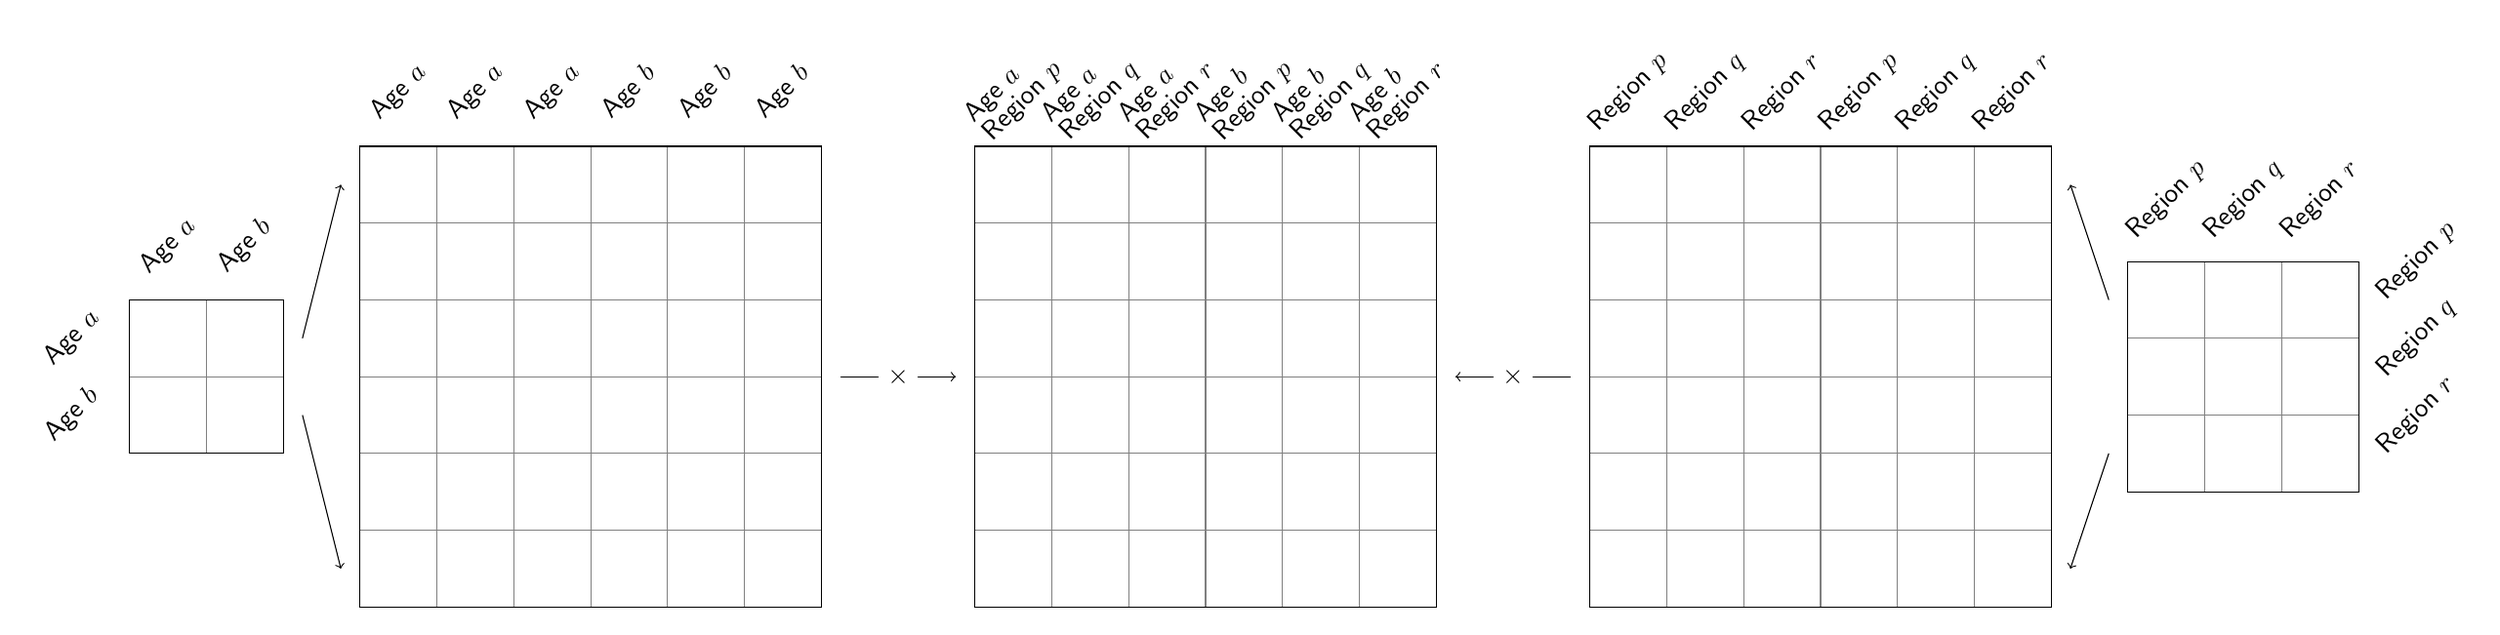
\begin{tikzpicture}
	% 2 x 2 age matrix
	\draw [color = grey] (0, 3) rectangle (1, 4);
	\draw [color = grey] (1, 3) rectangle (2, 4);
	% Second row
	\draw [color = grey] (0, 2) rectangle (1, 3);
	\draw [color = grey] (1, 2) rectangle (2, 3);
	% Top labels
	\node [align = left, rotate = 45, font = \linespread{0.8}\selectfont] at (0.5, 4.7) {Age $a$};
	\node [align = left, rotate = 45, font = \linespread{0.8}\selectfont] at (1.5, 4.7) {Age $b$};
	% Side labels
	\node [align = center, rotate = 45, font = \linespread{0.8}\selectfont] at (- 0.75, 3.5) {Age $a$};
	\node [align = center, rotate = 45, font = \linespread{0.8}\selectfont] at (- 0.75, 2.5) {Age $b$};
	% Edge
	\draw (0, 2) rectangle (2, 4);
	% Arrows
	\draw [->] (2.25, 3.5) -- (2.75, 5.5);
	\draw [->] (2.25, 2.5) -- (2.75, 0.5);
	
	% 6 x 6 age matrix 
	\draw [color = grey] (3, 5) rectangle (4, 6);
	\draw [color = grey] (4, 5) rectangle (5, 6);
	\draw [color = grey] (5, 5) rectangle (6, 6);
	\draw [color = grey] (6, 5) rectangle (7, 6);
	\draw [color = grey] (7, 5) rectangle (8, 6);
	\draw [color = grey] (8, 5) rectangle (9, 6);
	% Second row
	\draw [color = grey] (3, 4) rectangle (4, 5);
	\draw [color = grey] (4, 4) rectangle (5, 5);
	\draw [color = grey] (5, 4) rectangle (6, 5);
	\draw [color = grey] (6, 4) rectangle (7, 5);
	\draw [color = grey] (7, 4) rectangle (8, 5);
	\draw [color = grey] (8, 4) rectangle (9, 5);
	% Third row
	\draw [color = grey] (3, 3) rectangle (4, 4);
	\draw [color = grey] (4, 3) rectangle (5, 4);
	\draw [color = grey] (5, 3) rectangle (6, 4);
	\draw [color = grey] (6, 3) rectangle (7, 4);
	\draw [color = grey] (7, 3) rectangle (8, 4);
	\draw [color = grey] (8, 3) rectangle (9, 4);
	% Fourth row
	\draw [color = grey] (3, 2) rectangle (4, 3);
	\draw [color = grey] (4, 2) rectangle (5, 3);
	\draw [color = grey] (5, 2) rectangle (6, 3);
	\draw [color = grey] (6, 2) rectangle (7, 3);
	\draw [color = grey] (7, 2) rectangle (8, 3);
	\draw [color = grey] (8, 2) rectangle (9, 3);
	% Fifth row
	\draw [color = grey] (3, 1) rectangle (4, 2);
	\draw [color = grey] (4, 1) rectangle (5, 2);
	\draw [color = grey] (5, 1) rectangle (6, 2);
	\draw [color = grey] (6, 1) rectangle (7, 2);
	\draw [color = grey] (7, 1) rectangle (8, 2);
	\draw [color = grey] (8, 1) rectangle (9, 2);
	% Sixth row
	\draw [color = grey] (3, 0) rectangle (4, 1);
	\draw [color = grey] (4, 0) rectangle (5, 1);
	\draw [color = grey] (5, 0) rectangle (6, 1);
	\draw [color = grey] (6, 0) rectangle (7, 1);
	\draw [color = grey] (7, 0) rectangle (8, 1);
	\draw [color = grey] (8, 0) rectangle (9, 1);
	% Top labels
	\node [align = left, rotate = 45, font = \linespread{0.8}\selectfont] at (3.5, 6.7) {Age $a$};
	\node [align = left, rotate = 45, font = \linespread{0.8}\selectfont] at (4.5, 6.7) {Age $a$};
	\node [align = left, rotate = 45, font = \linespread{0.8}\selectfont] at (5.5, 6.7) {Age $a$};
	\node [align = left, rotate = 45, font = \linespread{0.8}\selectfont] at (6.5, 6.7) {Age $b$};
	\node [align = left, rotate = 45, font = \linespread{0.8}\selectfont] at (7.5, 6.7) {Age $b$};
	\node [align = left, rotate = 45, font = \linespread{0.8}\selectfont] at (8.5, 6.7) {Age $b$};
	% Edge
	\draw (3, 0) rectangle (9, 6);
	% Arrow
	\draw[->] (9.25, 3) -- (10.75, 3) node[pos = 0.5, fill = white] {$\times$};
	
	% 6 x 6 age and region matrix
	\draw [color = grey] (11, 5) rectangle (12, 6);
	\draw [color = grey] (12, 5) rectangle (13, 6);
	\draw [color = grey] (13, 5) rectangle (14, 6);
	\draw [color = grey] (14, 5) rectangle (15, 6);
	\draw [color = grey] (15, 5) rectangle (16, 6);
	\draw [color = grey] (16, 5) rectangle (17, 6);
	% Second row
	\draw [color = grey] (11, 4) rectangle (12, 5);
	\draw [color = grey] (12, 4) rectangle (13, 5);
	\draw [color = grey] (13, 4) rectangle (14, 5);
	\draw [color = grey] (14, 4) rectangle (15, 5);
	\draw [color = grey] (15, 4) rectangle (16, 5);
	\draw [color = grey] (16, 4) rectangle (17, 5);
	% Third row
	\draw [color = grey] (11, 3) rectangle (12, 4);
	\draw [color = grey] (12, 3) rectangle (13, 4);
	\draw [color = grey] (13, 3) rectangle (14, 4);
	\draw [color = grey] (14, 3) rectangle (15, 4);
	\draw [color = grey] (15, 3) rectangle (16, 4);
	\draw [color = grey] (16, 3) rectangle (17, 4);
	% Fourth row
	\draw [color = grey] (11, 2) rectangle (12, 3);
	\draw [color = grey] (12, 2) rectangle (13, 3);
	\draw [color = grey] (13, 2) rectangle (14, 3);
	\draw [color = grey] (14, 2) rectangle (15, 3);
	\draw [color = grey] (15, 2) rectangle (16, 3);
	\draw [color = grey] (16, 2) rectangle (17, 3);
	% Fifth row
	\draw [color = grey] (11, 1) rectangle (12, 2);
	\draw [color = grey] (12, 1) rectangle (13, 2);
	\draw [color = grey] (13, 1) rectangle (14, 2);
	\draw [color = grey] (14, 1) rectangle (15, 2);
	\draw [color = grey] (15, 1) rectangle (16, 2);
	\draw [color = grey] (16, 1) rectangle (17, 2);
	% Sixth row
	\draw [color = grey] (11, 0) rectangle (12, 1);
	\draw [color = grey] (12, 0) rectangle (13, 1);
	\draw [color = grey] (13, 0) rectangle (14, 1);
	\draw [color = grey] (14, 0) rectangle (15, 1);
	\draw [color = grey] (15, 0) rectangle (16, 1);
	\draw [color = grey] (16, 0) rectangle (17, 1);
	% Top labels
	\node [align = left, rotate = 45, font = \linespread{0.8}\selectfont] at (11.5, 6.7) {Age $a$\\ Region $p$};
    \node [align = left, rotate = 45, font = \linespread{0.8}\selectfont] at (12.5, 6.7) {Age $a$ \\ Region $q$};
	\node [align = left, rotate = 45, font = \linespread{0.8}\selectfont] at (13.5, 6.7) {Age $a$ \\ Region $r$};
	\node [align = left, rotate = 45, font = \linespread{0.8}\selectfont] at (14.5, 6.7) {Age $b$ \\ Region $p$};
	\node [align = left, rotate = 45, font = \linespread{0.8}\selectfont] at (15.5, 6.7) {Age $b$ \\ Region $q$};
	\node [align = left, rotate = 45, font = \linespread{0.8}\selectfont] at (16.5, 6.7) {Age $b$ \\ Region $r$};
    % Edge
	\draw (11, 0) rectangle (17, 6);
	% Arrow
	\draw[<-] (17.25, 3) -- (18.75, 3) node[pos = 0.5, fill = white] {$\times$};
	
	% 6 x 6 region and region matrix
	\draw [color = grey] (19, 5) rectangle (20, 6);
	\draw [color = grey] (20, 5) rectangle (21, 6);
	\draw [color = grey] (21, 5) rectangle (22, 6);
	\draw [color = grey] (22, 5) rectangle (23, 6);
	\draw [color = grey] (23, 5) rectangle (24, 6);
	\draw [color = grey] (24, 5) rectangle (25, 6);
	% Second row
	\draw [color = grey] (19, 4) rectangle (20, 5);
	\draw [color = grey] (20, 4) rectangle (21, 5);
	\draw [color = grey] (21, 4) rectangle (22, 5);
	\draw [color = grey] (22, 4) rectangle (23, 5);
	\draw [color = grey] (23, 4) rectangle (24, 5);
	\draw [color = grey] (24, 4) rectangle (25, 5);
	% Third row
	\draw [color = grey] (19, 3) rectangle (20, 4);
	\draw [color = grey] (20, 3) rectangle (21, 4);
	\draw [color = grey] (21, 3) rectangle (22, 4);
	\draw [color = grey] (22, 3) rectangle (23, 4);
	\draw [color = grey] (23, 3) rectangle (24, 4);
	\draw [color = grey] (24, 3) rectangle (25, 4);
	% Fourth row
	\draw [color = grey] (19, 2) rectangle (20, 3);
	\draw [color = grey] (20, 2) rectangle (21, 3);
	\draw [color = grey] (21, 2) rectangle (22, 3);
	\draw [color = grey] (22, 2) rectangle (23, 3);
	\draw [color = grey] (23, 2) rectangle (24, 3);
	\draw [color = grey] (24, 2) rectangle (25, 3);
	% Fifth row
	\draw [color = grey] (19, 1) rectangle (20, 2);
	\draw [color = grey] (20, 1) rectangle (21, 2);
	\draw [color = grey] (21, 1) rectangle (22, 2);
	\draw [color = grey] (22, 1) rectangle (23, 2);
	\draw [color = grey] (23, 1) rectangle (24, 2);
	\draw [color = grey] (24, 1) rectangle (25, 2);
	% Sixth row
	\draw [color = grey] (19, 0) rectangle (20, 1);
	\draw [color = grey] (20, 0) rectangle (21, 1);
	\draw [color = grey] (21, 0) rectangle (22, 1);
	\draw [color = grey] (22, 0) rectangle (23, 1);
	\draw [color = grey] (23, 0) rectangle (24, 1);
	\draw [color = grey] (24, 0) rectangle (25, 1);
	% Top labels
	\node [align = left, rotate = 45, font = \linespread{0.8}\selectfont] at (19.5, 6.7) {Region $p$};
	\node [align = left, rotate = 45, font = \linespread{0.8}\selectfont] at (20.5, 6.7) {Region $q$};
	\node [align = left, rotate = 45, font = \linespread{0.8}\selectfont] at (21.5, 6.7) {Region $r$};
	\node [align = left, rotate = 45, font = \linespread{0.8}\selectfont] at (22.5, 6.7) {Region $p$};
	\node [align = left, rotate = 45, font = \linespread{0.8}\selectfont] at (23.5, 6.7) {Region $q$};
	\node [align = left, rotate = 45, font = \linespread{0.8}\selectfont] at (24.5, 6.7) {Region $r$};
	% Edge
	\draw (19, 0) rectangle (25, 6);
	
	% 3 x 3 region matrix
	\draw [color = grey] (26, 3.5) rectangle (27, 4.5);
	\draw [color = grey] (27, 3.5) rectangle (28, 4.5);
	\draw [color = grey] (28, 3.5) rectangle (29, 4.5);
	% Second row
	\draw [color = grey] (26, 2.5) rectangle (27, 3.5);
	\draw [color = grey] (27, 2.5) rectangle (28, 3.5);
	\draw [color = grey] (28, 2.5) rectangle (29, 3.5);
	% Third row
	\draw [color = grey] (26, 1.5) rectangle (27, 2.5);
	\draw [color = grey] (27, 1.5) rectangle (28, 2.5);
	\draw [color = grey] (28, 1.5) rectangle (29, 2.5);
	% Top labels
	\node [align = left, rotate = 45, font = \linespread{0.8}\selectfont] at (26.5, 5.3) {Region $p$};
	\node [align = left, rotate = 45, font = \linespread{0.8}\selectfont] at (27.5, 5.3) {Region $q$};
	\node [align = left, rotate = 45, font = \linespread{0.8}\selectfont] at (28.5, 5.3) {Region $r$};
	% Side labels
	\node [align = center, rotate = 45, font = \linespread{0.8}\selectfont] at (29.75, 4.5) {Region $p$};
	\node [align = center, rotate = 45, font = \linespread{0.8}\selectfont] at (29.75, 3.5) {Region $q$};
	\node [align = center, rotate = 45, font = \linespread{0.8}\selectfont] at (29.75, 2.5) {Region $r$};
	% Edge
	\draw (26, 1.5) rectangle (29, 4.5);
	% Arrows
	\draw [<-] (25.25, 5.5) -- (25.75, 4);
	\draw [<-] (25.25, 0.5) -- (25.75, 2);
\end{tikzpicture}
\end{document}
